\documentclass{beamer}
\usetheme{Boadilla}
\setbeamertemplate{navigation symbols}{} % To remove the navigation symbols from the bottom of all slides uncomment this line

%------------------------------------------------
% Colors
\usepackage{xcolor}	 % Required for custom colors
% Define a few colors for making text stand out within the presentation
\definecolor{mygreen}{RGB}{44,85,17}
\definecolor{myblue}{RGB}{34,31,217}
\definecolor{mybrown}{RGB}{194,164,113}
\definecolor{myred}{RGB}{255,66,56}
% Use these colors within the presentation by enclosing text in the commands below
\newcommand*{\mygreen}[1]{\textcolor{mygreen}{#1}}
\newcommand*{\myblue}[1]{\textcolor{myblue}{#1}}
\newcommand*{\mybrown}[1]{\textcolor{mybrown}{#1}}
\newcommand*{\myred}[1]{\textcolor{myred}{#1}}
%------------------------------------------------
\setbeamercolor{structure}{fg=mygreen}
%------------------------------------------------
\setbeamertemplate{itemize item}{\scriptsize\raise1.25pt\hbox{\donotcoloroutermaths$\blacktriangleright$}}
\setbeamertemplate{itemize subitem}{\tiny\raise1.5pt\hbox{\donotcoloroutermaths$\blacktriangleright$}}
\setbeamertemplate{itemize subsubitem}{\tiny\raise1.5pt\hbox{\donotcoloroutermaths$\blacktriangleright$}}


%------------------------------------------------
% Fonts
%------------------------------------------------
\usepackage[T1]{fontenc}	 % For correct hyphenation and T1 encoding
\usepackage{lmodern} % Default font: latin modern font
\renewcommand{\familydefault}{\sfdefault} % Sans serif - this may need to be commented to see the alternative fonts
%------------------------------------------------

%------------------------------------------------
% Various required packages
%-----------------------------------------------
\usepackage{graphicx} % Required for including images in figures
\usepackage{booktabs} % Required for horizontal rules in tables
\usepackage{multicol} % Required for creating multiple columns in slides
\usepackage[english]{babel} % Document language - required for customizing section titles
\usepackage{color}
\usepackage{booktabs} % Allows the use of \toprule, \midrule and \bottomrule in tables
\usepackage{multicol}
\usepackage{textpos}
\usepackage{tikz}
\usepackage{hyperref}
\usepackage{multirow}
%------------------------------------------------
\newcommand{\topline}{%
  \tikz[remember picture,overlay] {%
    \draw[mygreen,very thick] ([yshift=-1.7cm]current page.north west)
             -- ([yshift=-1.7cm,xshift=11cm]current page.north west);}}
%------------------------------------------------
% Slide layout configuration

\setbeamertemplate{frametitle}
{	
	\huge
	\vspace*{0.3cm}
    \insertframetitle  \\
     \tikz[remember picture,overlay] {%
        \draw[mygreen,very thick] ([yshift=-1.7cm]current page.north west)
                 -- ([yshift=-1.7cm,xshift=11cm]current page.north west);}
     
  %  \insertframesubtitle
}
%\AtBeginDocument{\renewcaptionname{english}{\contentsname}{\Large Agenda}} 
%Title
%------------------------------------------------
\title[]{RETRIEVAL ADVANCES OF BrO/SO2 MOLAR RATIOS FROM NOVAC} % The short title appears at the bottom of every slide, the full title is only on the title page

\author{Elsa Wilken} % Your name
\institute[] % Your institution as it will appear on the bottom of every slide, may be shorthand to save space
{
Master Thesis \\ % Your institution for the title page
\medskip
%\textit{e.wilken@yahoo.de} % Your email address
}
\date{\today} % Date, can be changed to a custom date




\begin{document}

%------------------------------------------------
%	TITLE SLIDE
%------------------------------------------------
\begin{frame}
\titlepage
\end{frame}


%------------------------------------------------
%	Established Routine
%------------------------------------------------
\frame{
\frametitle{Established Routine}
\hspace*{-0.4cm}
\includegraphics[width=1.05\linewidth]{./Bilder/DOAS_Fit_Routine}
}
%------------------------------------------------
%	Contamination Problem
%------------------------------------------------
\frame{
\frametitle{Contamination Problem}
	\begin{multicols}{2}
		\begin{itemize}
			\item In total ca. 7$\%$  of the Data are contaminated 
		\end{itemize}
		In the following we only work with the contaminated data
		\begin{minipage}[t]{0.5\textwidth}
			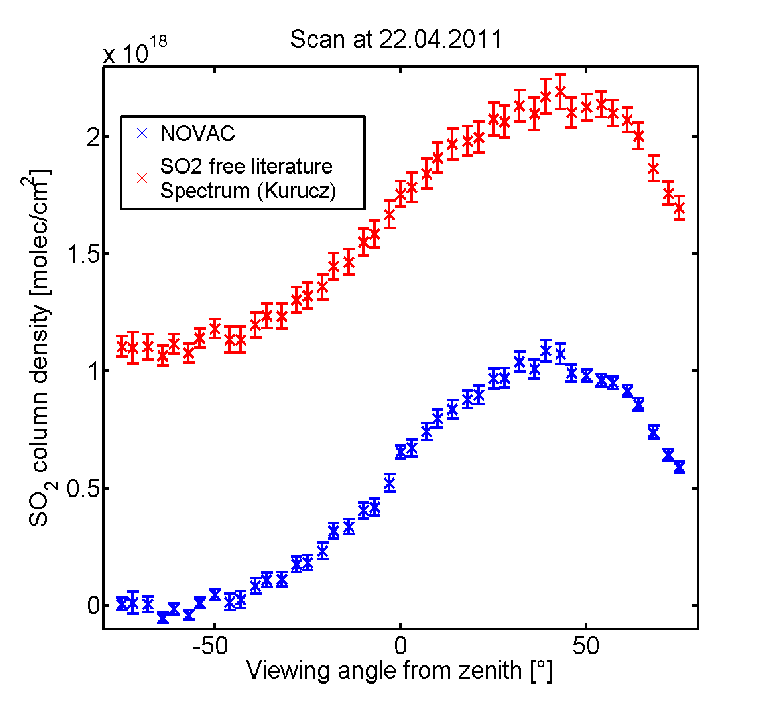
\includegraphics[width=\textwidth]{./Bilder/contaminated}
		\end{minipage}
	\end{multicols}
}
%------------------------------------------------
%	BrO Error dependency on variables
%------------------------------------------------
\frame{
\frametitle{BrO Error dependency on variables}
\begin{multicols}{2}
%
	\vspace*{-1.2cm}
	\begin{minipage}[t]{0.5\textwidth}
		\includegraphics[width=0.85\linewidth]{./Bilder/Differcence_in_Instrument_TemperatureC1}
	\end{minipage}
	%
	\vspace*{-0.4cm}
	\begin{minipage}[t]{0.5\textwidth}
		\includegraphics[width=0.85\linewidth]{./Bilder/Differcence_in_Day_Timeh1}
	\end{minipage}
	%
	\newpage
	\vspace*{-1.2cm}
	\begin{minipage}[t]{0.5\textwidth}
		\includegraphics[width=0.85\linewidth]{./Bilder/Differcence_in_ExposureTime_ms1}
	\end{minipage}
	%
	\vspace*{-0.4cm}
	\begin{minipage}[t]{0.5\textwidth}
		\includegraphics[width=0.85\linewidth]{./Bilder/Differcence_in_Colorindex1}
	\end{minipage}
%
\end{multicols}
}
%------------------------------------------------
%	Calculations
%------------------------------------------------
\frame{
\frametitle{Calculations}
\begin{itemize}
\item linear approximation of the Data
\end{itemize}
\vspace{1cm}
	\begin{equation*}
	\Delta	\epsilon_{BrO} = a_{t}\cdot\Delta t+a_{temp}\cdot\Delta temp+a_{daytime}\cdot\Delta daytime +a_{coloridx}\cdot\Delta coloridx
	\end{equation*}
}
%------------------------------------------------
%	Actual fit in python
%------------------------------------------------
%\frame{
%\frametitle{Actual fit in python}
%\begin{itemize}
%\item 
%\end{itemize}
%}

%------------------------------------------------
%	Importance of Variables
%------------------------------------------------
\frame{
\frametitle{Calculations}
	Hereby are the constants 
	\begin{table}[h]
		\begin{tabular}{c|c|c}
			\toprule
			Constant& importance& deviation\\
			\toprule
			$a_{T}$& 0.661 & 29$\%$\\
			\midrule
			$a_{ET}$&0.011&164$\%$\\
			\midrule
			$a_{t}$& 0.133&50$\%$\\
			\midrule
			$a_{dt}$&0.138&	65$\%$\\
			\midrule
			$a_{c}$&0.061&136$\%$\\
			\bottomrule
		\end{tabular}
	\end{table}
}
%------------------------------------------------
%	Results
%------------------------------------------------
\frame{
\frametitle{Results}
\begin{itemize}
\item Results only for contaminated data
\item Data are treated as contaminated if the SO2 column density is larger as $2\cdot10^{17}\quad \frac{molec}{cm^2}$
\item Plume data are reliable if the SO2 column density is larger as $7\cdot10^{17}\quad \frac{molec}{cm^2}$
\item The results are described relative to an optimal evaluation
\item The optimal Evaluation is done by choosing the smallest total error
\item If the relative error is larger than 5 we don't use the data
\end{itemize}

}
%------------------------------------------------
%	SO2 Evaluation
%------------------------------------------------
\frame{
\frametitle{SO2 Evaluation}
\begin{multicols}{2}
\begin{itemize}
\item Increase if the SO2 column densities of: 84$\%$
\begin{itemize}
\item PILLATE: 62$\%$
\item HUAYRAPATE: 122$\%$
\item BAYUSHIG: 23$\%$ (\small{very view data})

\end{itemize}

%\item Faktor um den der Fehler w\"achst: 1.89
\item More Data relative to the NOVAC-Evaluation: 206$\%$ 
\end{itemize}

\begin{minipage}[t]{0.5\textwidth}
\footnote{Fit uses only data where SO2 column \\
density is higher than $7\cdot 10^{17}\frac{molec}{cm^2}$}
\includegraphics[width=\textwidth]{./Bilder/SO2_comparison}
\end{minipage}
\end{multicols}
}
%------------------------------------------------
%	BrO Evaluation
%------------------------------------------------
\frame{
\frametitle{BrO Evalutaion}
\begin{multicols}{2}
\begin{itemize}
\item Instrument PILLATE
\begin{itemize}
\item Increase of BrO column density: 30$\%$
%\item Fehler:  1.67
%\item G\"ultige Daten: 80$\%$
\end{itemize}
\item Instrument HUAYRAPATE
\begin{itemize}
\item Increase of BrO column density: 87$\%$
%\item Fehler: 1.51
%\item G\"ultige Daten: 62$\%$
\end{itemize}
\item Instrument BAYUSHIG (\small{very view data})

\begin{itemize}
\item Increase of BrO column density: 35$\%$
%\item Fehler: 1.69
%\item keine g\"ultige Daten
\end{itemize}

\end{itemize}
\begin{minipage}[t]{0.5\textwidth}
\vspace*{-1cm}
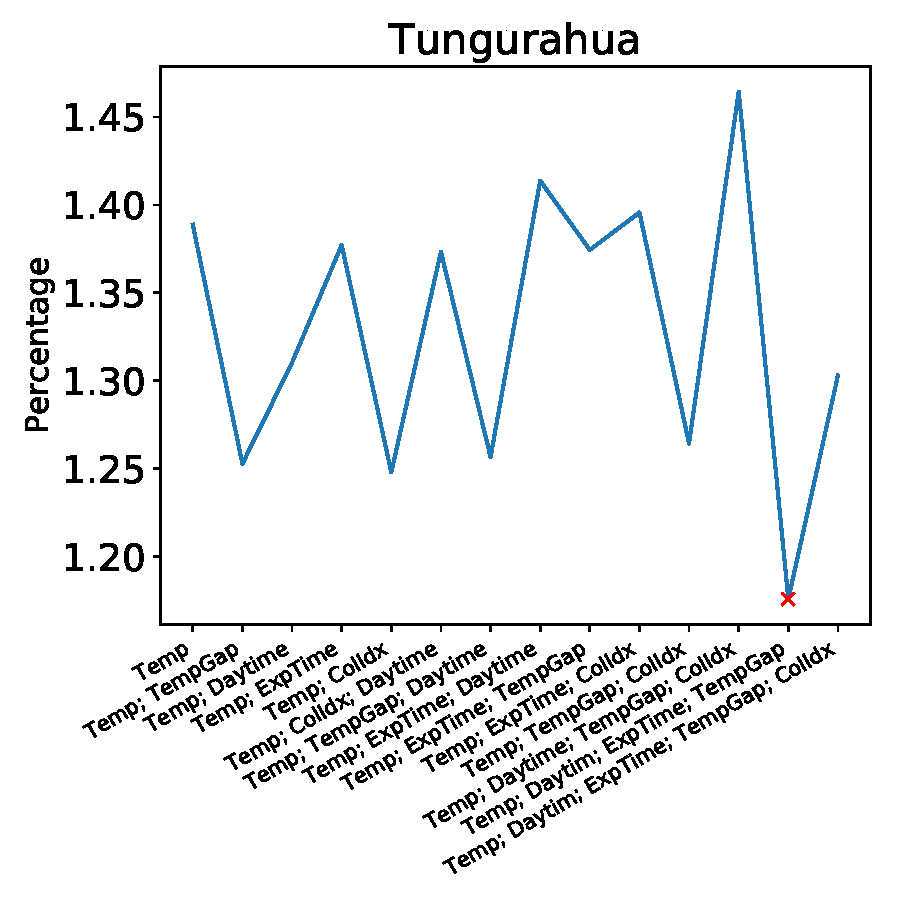
\includegraphics[width=0.9\textwidth]{./Bilder/Tungurahua}
\end{minipage}
\end{multicols}
}


\frame{
\frametitle{BrO Evaluation}
\begin{multicols}{2}
\begin{itemize}
\item Increase of BrO column density: 52$\%$
%\item More Data: 51$\%$
%\item More valid Data: 38$\%$ 
\item Factor the absolute error increases relative to the NOVAC-evaluation: 1.65
\item Factor the relative error increases relative to the optimal-results: 1.5
\end{itemize}

\begin{minipage}[t]{0.5\textwidth}
\footnote{Fit uses only data where SO2 column \\
density is higher than $7\cdot 10^{17}\frac{molec}{cm^2}$}
\includegraphics[width=\textwidth]{./Bilder/BrO_comparison}
\end{minipage}
\end{multicols}
}
\frame{
\frametitle{Other Methods}
	\begin{table}[h]
%		\begin{tabular}{|p{2cm}|p{2.5cm}|p{1.5cm}|p{1.5cm}||p{1cm}|}
%		%	\toprule
%			&& Error & Amount of Data&davon gültig\\
%			\toprule
%			\multirow{2}{5em}{All Variables} 
%				& independent& 1.51 & 95$\%$&10,5$\%$\\
%				& dependent & 1.40&176 &14\\
%			\midrule
%			\multirow{2}{5em}{Exposure Time}
%					&  independent &1.47&174&18\\
%					& All &1.39&176&13\\
%			\midrule
%			\multirow{2}{5em}{Exp.Time u Coloridx}
%					&  independent &1.4&175&20\\
%					& All &1.35&176&13\\
%			\bottomrule
%		\end{tabular}
		\begin{tabular}{|p{2cm}|p{2.5cm}|p{1.5cm}|p{1.5cm}||p{1cm}|}
		%	\toprule
			&& Error & Amount of Data&valid data\\
			\toprule
			\multirow{2}{5em}{All Variables} 
				& independent& 1.51 & 95$\%$&10,5$\%$\\
				& dependent & 1.40&98$\%$ &8$\%$\\
			\midrule
			\multirow{2}{5em}{Exposure Time}
					&  independent &1.47&97$\%$&10$\%$\\
					& All &1.39&98$\%$&7$\%$\\
			\midrule
			\multirow{2}{5em}{Exp.Time u Coloridx}
					&  independent &1.40& 98$\%$&11\\
					& All & 1.35& 98$\%$&7$\%$\\
			\bottomrule
		\end{tabular}
	\end{table}
	$\bullet$ In the optimal results are 15$\%$ valid data
}

%------------------------------------------------
%	BrO Evaluation
%------------------------------------------------
\frame{
\frametitle{Ratio Evaluation}
\begin{multicols}{2}
\begin{itemize}
\item Decrease of gas ratio: 25$\%$
\begin{itemize}
\item PILLATE: 32$\%$
\item HUAYRAPATE: 12$\%$
\item BAYUSHIG: -6$\%$(\small{very view data})

\end{itemize}
%\item Difference zwischen den Berechnungsmethoden sink mit der Zunahme des Gas-Verh\"altnisses.
\end{itemize}

\begin{minipage}[t]{0.5\textwidth}
\includegraphics[width=\textwidth]{./Bilder/Ratio_comparison}
\end{minipage}
\end{multicols}
}

\frame{
\frametitle{Total evaluation}
\begin{itemize}

\item More BrO Data: 51$\%$
\item More valid BrO Data: 38$\%$ 
%\item An average decrease of Ratio of 35$\%$

\end{itemize}
}


\end{document}
